\documentclass[handout]{beamer}
\usepackage{multicol}
\usepackage{xy}
\everymath{\displaystyle}
\mode<presentation>
{\usetheme{Warsaw}\setbeamercovered{dynamic}}
\usecolortheme{crane}
\usepackage{beamerfoils}
\pgfdeclareimage[height=1in]{university-logo}{ISULogo}
\logo{\pgfuseimage{university-logo}}
\setbeamertemplate{navigation symbols}{}
\title[\S6]{Section 6\\{\em And} and {\em or} problems}
\author{Dr Marcus Bishop}
\subject{Math 104}
\beamerdefaultoverlayspecification{<+->}
\theoremstyle{definition}
\newtheorem{remark}{Remark}
\newtheorem{impact}{Impact}
\newtheorem{notation}{Notation}
\usepackage{arev}
\begin{document}
\begin{frame}\titlepage\end{frame}
\LogoOff

\begin{frame}{Card problem from exam}
\begin{itemize}
\item How many cards either are picture cards or have
suit \alert{$\varheart$}?
\item Observe that thirteen cards have
suit \alert{$\varheart$}, namely
\[A\alert{\varheart},
2\alert{\varheart},
3\alert{\varheart},\ldots,
10\alert{\varheart},
J\alert{\varheart},
Q\alert{\varheart},
K\alert{\varheart}\]
\item Observe that twelve cards are picture cards, namely
\[J\alert{\varheart},J\alert{\vardiamond},J\clubsuit,J\spadesuit,
Q\alert{\varheart},Q\alert{\vardiamond},Q\clubsuit,Q\spadesuit,
K\alert{\varheart},K\alert{\vardiamond},K\clubsuit,K\spadesuit\]
\item However, \alert{three} cards in both groups,
namely
\[J\alert{\varheart},Q\alert{\varheart},K\alert{\varheart}\]
\item Thus $13+12-3=22$ cards are either picture cards or have 
suit \alert{$\varheart$}
\end{itemize}
\end{frame}

\begin{frame}{Inclusion-Exclusion Formula}
\begin{theorem}[Inclusion-Exclusion Formula]
Suppose that
\begin{itemize}
\item $M$ has $m$ elements 
\item $N$ has $n$ elements
\item There are $p$ elements in \alert{both} $M$ and $N$
\end{itemize}
Then there are $m+n-p$ elements in \alert{either} $M$ or $N$
\end{theorem}
\end{frame}

\begin{frame}{Example}
\begin{itemize}
\item How many of $1,2,\ldots,12$ are
either divisible by $3$ or greater than $6$?
\item Numbers divisible by $3$: $3,6,9,12$
\item Numbers greater than $6$: $7,8,9,10,11,12$
\item Numbers in both groups: $9,12$
\item Thus $4+6-2=8$
either divisible by $3$ or greater than $6$?
\end{itemize}
\end{frame}

\begin{frame}{Venn diagrams}
\begin{itemize}
\item Can visualize last example using Venn diagram:
\[\begin{xy}<1cm,0cm>:
(-1,0)*\cir<2cm>{};
(1,0)*\cir<2cm>{};
(-1.5,1)*{3};
(-1.5,-1)*{6};
(0,1)*{9};
(0,-1)*{12};
(1.25,1)*{7};
(1.25,-1)*{10};
(2,1)*{8};
(2,-1)*{11};
\end{xy}\]
\item Numbers divisible by $3$ in left circle
\item Numbers greater than $6$ in right circle
\item Numbers in both groups in both circles
\end{itemize}
\end{frame}

\begin{frame}{Greek, Roman, Russian alphabets}
\begin{multicols}{2}
\begin{itemize}
\item Upper left circle shows letters of Greek alphabet
\item Upper right circle shows letters of Roman alphabet
\item Lower circle shows letters of Russian alphabet
\item How many in Roman and Russian but not Greek?
\only<+->{One, namely C}
\item How many letters in all three?
\only<+->{11}
\end{itemize}
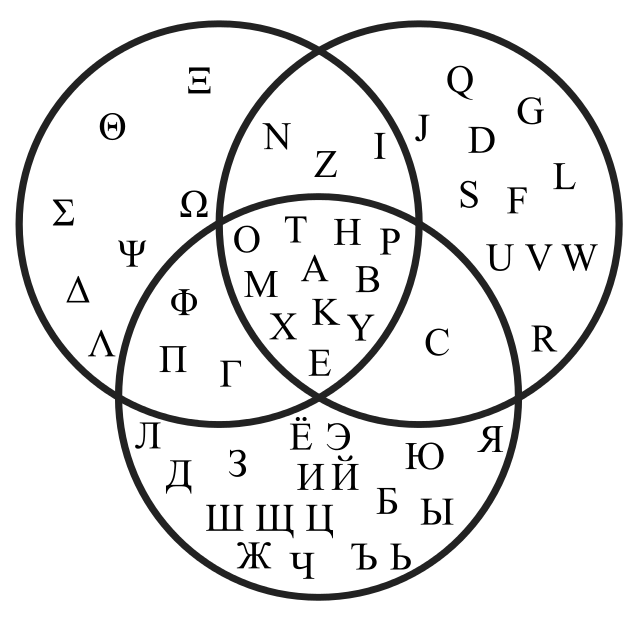
\includegraphics[scale=.25]{Venn}
\end{multicols}
\end{frame}

\begin{frame}{Freshman music majors}
\begin{itemize}
\item $100$ freshman majoring in (instrumental) music
required to be in either band or orchestra
\item $75$ in band
\item $35$ in both band and orchestra
\item How many in orchestra?
\item Rather than drawing freshmen in circles,
write only \alert{number} of freshman in each
group in corresponding region 
\[\begin{xy}<1cm,0cm>:
(-1,2)*+!D{\text{Band}};
(1,2)*+!D{\text{Orch}};
(-1,0)*\cir<2cm>{};
(1,0)*\cir<2cm>{};
(0,0)*{35};
\end{xy}\]
\end{itemize}
\end{frame}

\begin{frame}
\begin{itemize}
\item Since $75$ in band, must have
$40$ in band but not orchestra:
\[\begin{xy}<1cm,0cm>:
(-1,2)*+!D{\text{Band}};
(1,2)*+!D{\text{Orch}};
(-1,0)*\cir<2cm>{};
(1,0)*\cir<2cm>{};
(0,0)*{35};
(-2,0)*{40};
\end{xy}\]
\end{itemize}
\end{frame}

\begin{frame}
\begin{itemize}
\item Must be $100-75=25$ in orchestra but not band:
\[\begin{xy}<1cm,0cm>:
(-1,2)*+!D{\text{Band}};
(1,2)*+!D{\text{Orch}};
(-1,0)*\cir<2cm>{};
(1,0)*\cir<2cm>{};
(0,0)*{35};
(-2,0)*{40};
(2,0)*{25};
\end{xy}\]
\item Thus $35+25=60$ in orchestra
\end{itemize}
\begin{remark}
Solving Inclusion Exclusion Formula
\[75+n-35=100\]
for $n$ obviates Venn diagram
\end{remark}
\end{frame}

\begin{frame}{More Inclusion-Exclusion}
\begin{theorem}[Inclusion-Exclusion Formula]
If $E,F$ events and
\begin{itemize}
\item $p=P\left(E\right)$
\item $q=P\left(F\right)$
\item $r$ the probability that \alert{both} $E$ and $F$ occur
\end{itemize}
then $p+q-r$ the probability that \alert{either} $E$ or $F$ occurs
\end{theorem}
\begin{example}[Exercise 11]
\begin{itemize}
\item Suppose $P\left(E\right)=0.8$,
$P\left(F\right)=0.5$, and $P\left(\text{$E$ and $F$}\right)=0.5$
\item Then $P\left(\text{$E$ or $F$}\right)
=0.8+0.4-0.5=0.7$
\item Example doesn't even require context
\end{itemize}
\end{example}
\end{frame}

\begin{frame}{Example}
\begin{itemize}
\item Recall that $3,6,9,12$ divisible by $3$
\item So if number randomly selected from
$1,2,\ldots,12$ then $4/12$
the probability number divisible by $3$
\item Similarly $7,8,9,10,11,12$ greater than $6$
\item So $6/12$ the probability number
greater than $6$
\item Finally, $9,12$ divisible by $3$ \alert{and}
greater than $6$
\item So $2/12$ the probability that number
both divisible by $3$ and greater than $6$
\item By Inclusion-Exclusion
\[\frac{4}{12}+\frac{6}{12}-\frac{2}{12}=\frac{8}{12}\]
the probability
that number \alert{either} divisible by $3$ or greater than $6$
\item Indeed eight numbers $3,6,7,8,9,10,11,12$ 
divisible by $3$ or greater than $6$
\end{itemize}
\end{frame}

\begin{frame}{Mutually exclusive events}
\begin{itemize}
\item If Then $0=P\left(\text{$E$ and $F$}\right)$
then $E,F$ called \alert{mutually exclusive events}
\item Means that impossible for \alert{both} $E$ and $F$ to occur
\end{itemize}
\begin{example}
\begin{itemize}
\item Experiment: roll die
\item $E=\left\{1,3,5\right\}$, the event
that odd number rolled
\item $F=\left\{2,4,6\right\}$, the event
that even number rolled
\item Then $E,F$ mutually exclusive
\item Note that as sets, $E,F$ have \alert{no elements} in common
\end{itemize}
\end{example}
\begin{example}
\begin{itemize}
\item But mutually exclusive events need not be \alert{complementary}
\item $E=\left\{1,3,5\right\}$ and $F=\left\{2\right\}$
mutually exclusive
\end{itemize}
\end{example}
\end{frame}

\begin{frame}
\begin{itemize}
\item Note that if $E,F$ mutually exclusive then Inclusion-Exclusion
formula reduces to
\[P\left(\text{$E$ or $F$}\right)=P\left(E\right)
+P\left(F\right)\alert{-0}\]
since $0=P\left(\text{$E$ and $F$}\right)$
\end{itemize}
\begin{example}
\begin{itemize}
\item Experiment: randomly select card
\item $P\left(\clubsuit\right)=\frac{1}{4}=P\left(\alert{\varheart}\right)$
\item $\clubsuit,\alert{\varheart}$ mutually exclusive
since no card has \alert{both} suits
\item Thus $P\left(\text{$\clubsuit$ or $\alert{\varheart}$}\right)
=\frac{1}{4}+\frac{1}{4}=\frac{1}{2}$
\end{itemize}
\end{example}
\end{frame}


\end{document}
